\section{Summarization model}
In this part we implements and fine-tunes Google's PEGASUS (Pre-training with Extracted Gap-sentences for Abstractive SUmmarization) model for automatic text summarization, specifically targeting dialogue summarization using the SAMSum dataset. The implementation leverages state-of-the-art transformer architecture to convert conversational dialogues into concise, coherent summaries.
\subsection{Dataset}
We choose the \href{https://huggingface.co/datasets/knkarthick/samsum}{The SAMSum dataset (knkarthick/samsum)} for fine tuning this model due to the following reasons:
\begin{itemize}
    \item Scale: 14,732 training conversations, 818 validation, 819 test samples
    \item Human-written summaries ensure high-quality supervision
    \item Covers various conversation types, topics, and communication styles
    \item Authentic dialogue patterns reflecting real-world conversational structures
\end{itemize}
\subsubsection{Results}
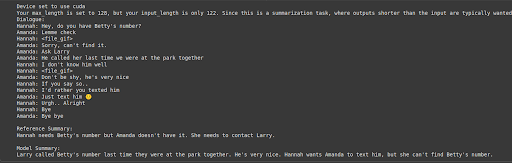
\includegraphics[scale = 0.9]{experiements/image/result1.png}
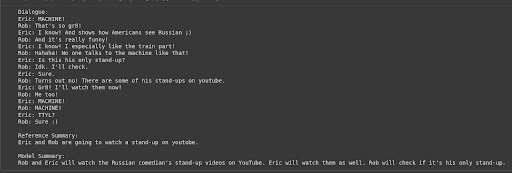
\includegraphics[scale = 0.9]{experiements/image/result2.png}

